%*********************************************************************
% gdutthesis: 广东工业大学论文模板
% 2025/02/09 v0.1f
%
% 重要提示:
%   1. 请确保使用 UTF-8 编码保存
%   2. 请使用 XeLaTeX 或 LuaLaTeX 编译:建议先用 XeLaTeX 编译一次,再用 BibTeX 编译一次,最后再用 XeLaTeX 编译两次
%   3. 请仔细阅读用户文档和 Wiki
%   4. 修改、使用、发布本文档请务必遵循 LaTeX Project Public License
%   5. 不需要的注释可以尽情删除
%   6. 请使用最新版本的模板并在打印前检查输入信息与学校要求是否一致
%*********************************************************************
\documentclass[
  % type=doctor
  % type=master
  type=promaster  % 专业学位
]{gdutthesis}

% 宏包在这里加载
\usepackage{siunitx}[=v2]
\usepackage{zhlipsum,lipsum}

\gdutsetup{
  style = {
    cover           = {true},
    open            = {true},
    % open            = {false},
    free-float      = {true},
    % free-float      = {false},
    % font            = {garamond},
    % font            = {libertinus},
    % font            = {lm},
    % font            = {palatino},
    font            = {times},
    % font            = {times*},
    % math-font       = {garamond},
    % math-font       = {libertinus},
    % math-font       = {lm},
    % math-font       = {palatino},
    math-font       = {times},
    % math-font       = {times*},
    % cjk-font        = {fandol},
    % cjk-font        = {founder},
    % cjk-font        = {mac},
    % cjk-font        = {sourcehan},
    % cjk-font        = {noto},
    cjk-font        = {windows},
    % cjk-font        = {none},
    bib-backend     = {bibtex},
    % bib-backend     = {biblatex},
    bib-resource    = {ref/gdutthesis-template.bib, ref/reference.bib},
    bib-style       = {numerical},
    % bib-style       = {author-year},
    % fullwidth-stop  = {mapping},
    % fullwidth-stop  = {catcode},
    fullwidth-stop  = {false},
    hyperlink       = {color},
    % hyperlink       = {border},
    % hyperlink       = {none},
    hyperlink-color = {default},
    % hyperlink-color = {autumn},
    % hyperlink-color = {business},
    % hyperlink-color = {classic},
    % hyperlink-color = {elegant},
    % hyperlink-color = {fantasy},
    % hyperlink-color = {material},
    % hyperlink-color = {science},
    % hyperlink-color = {summer},
    % hyperlink-color = {graylevel},
    % hyperlink-color = {prl},
  },
  theorem = {
    header-font = bf,
    % header-font = sf,
    body-font   = rm,
    % body-font   = kai,
    indent      = cn,
    % indent      = en,
    interval    = dash,
    % interval    = dot,
    braces      = paren,
    % braces      = bracket,
    punct       = colon,
    % punct       = quad,
    qed         = \qedsymbol,
    % qed         = \QED,
  },
  info = {
    title             = {这是论文标题},
    title*            = {This is the title of the thesis},
    date              = {2025/5/25},
    author            = {作者},
    author*           = {author},
    supervisor        = {导师一, 教授},
    supervisor*       = {supervisor-one},
    supervisor-two    = {导师二, 副教授},
    supervisor-two*   = {supervisor-two},
    supervisor-three  = {导师三, 副教授},
    supervisor-three* = {supervisor-three},
    supervisor-out    = {校外导师, 研究员},
    supervisor-out*   = {supervisor-out},
    department        = {环境科学与工程学院},
    department*       = {School of Environmental Science and Engineering},
    major             = {环境工程},
    student-id        = {2112210000},
    chairman          = {答辩主席},
    degree            = {工程硕士},
    degree*           = {Master of Engineering Science},
    keywords          = {关键词一, 关键词二, 关键词三},
    keywords*         = {keyword-one, keyword-two, keyword-three},
    secret-level      = {none},
    delay-time        = {none},
  }
}


\begin{document}

\gdutstatement % 空白声明页
% \gdutstatement[日期][作者签名][导师签名]% 签名为图片
% \gdutstatement*[扫描件]% 扫描件为 A4 大小的 pdf 文件

\begin{abstract}
  \zhlipsum[1]
\end{abstract}

\begin{abstract*}
  \zhlipsum[1]
\end{abstract*}

\begin{notation}
  \toprule
  符号  & 含义 \\
  \midrule
  $E$   & 能量 \\
  $F$   & 推力 \\
  \bottomrule
\end{notation}

\printnoidxglossaries

\gduttableofcontents

\mainmatter

\chapter{绪论}{Introduction}

\section{本课题研究背景及研究意义}{Background and significance of research}

\zhlipsum[1]

\section{国内外相关研究现状}{Analysis of the research status at home and abroad}

\subsection{测试}{test}

测试\gdutcite{chendengyuan2000guoshi},测试\gdutcite*{woerdelun2012jingji}。

测试如\autoref{fig:example} 所示,具体参考\autoref{sub-fig-1} 和\autoref{sub-fig-2}。

测试参考\autoref{eq:example}。

测试参考\autoref{tab:example}。

测试\gls{slm},\gls{slm},\gls{glm},\gls{glm}。

\subsubsection{测试}
测试 test。
\paragraph{测试 test。}
测试 test。
\subparagraph{测试 test。}
测试 test。

% 大部分情况使用 align/gather 环境,小部分间距异常情况可尝试使用 equation 环境
\begin{align}
  E &= mc^2 \label{eq:example} \\
  mc^2 &= E
\end{align}

\begin{gather}
  E = mc^2 \\
  mc^2 = E
\end{gather}

\begin{figure}
  \subfloat[贴有模板的金属喷嘴示意图]{\label{sub-fig-1}
    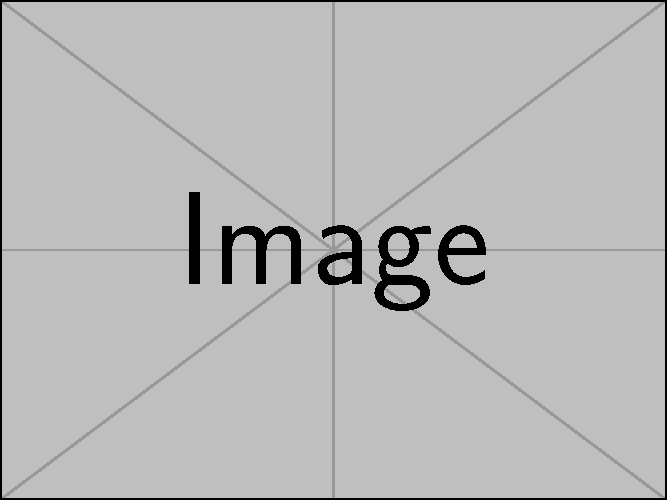
\includegraphics[width=0.4\textwidth]{example-image.pdf}
  }
  \qquad
  \subfloat[由点到线扫描加工原理图]{\label{sub-fig-2}
    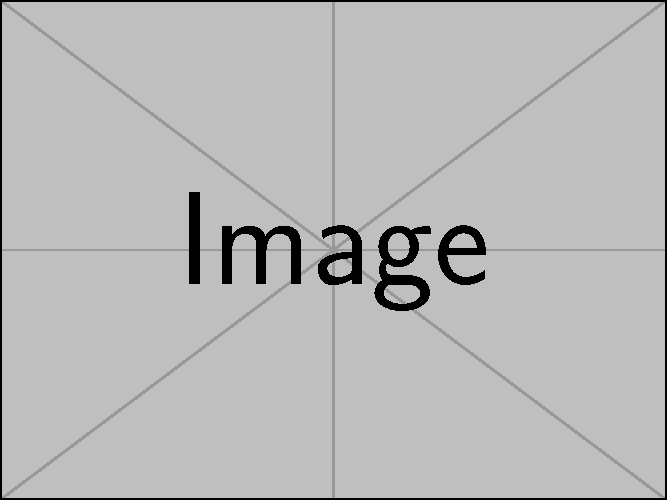
\includegraphics[width=0.4\textwidth]{example-image.pdf}
  }
  \bicaption{模板射流电解加工微沟槽原理图}{Principle of masked jet electrochemical machining of micro grooves}
  \label{fig:example}
\end{figure}

\begin{table}
  \bicaption{DMC5400A 运动控制卡主要技术指标}{DMC5400A main specifications}
  \label{tab:example}
  \begin{tabular}{cc}
    \toprule
    控制卡技术指标              & 具体参数                      \\
    \midrule
    控制电机的脉冲信号频率范围  & $\SI{1}{Hz}\sim\SI{2}{MHz}$   \\
    控制电机的脉冲信号频率精度  & \SI{0.0625}{Hz}               \\
    脉冲信号输出最大电流        & \SI{20}{mA}                   \\
    脉冲信号长度                & 28 位有符号                   \\
    直线插补精度                & $\pm \SI{0.8}{pulse}$         \\
    圆弧插补精度                & $\pm \SI{1.5}{pulse}$         \\
    支持的插补坐标系个数        & 2                             \\
    \bottomrule
  \end{tabular}
\end{table}

\chapter{结论与展望}{Conclusion and prospect}
\gdutbacksection{研究结论}
\zhlipsum[1]

\gdutbacksection{未来研究展望}
\zhlipsum[1]

\gdutbackmatter

\nocite{*}% 列出 bib 文件中的全部参考文献
\printbibliography

\chapter{攻读学位期间取得的相关成果}{Publications and patents during study}

\gdutbacksection{攻读学位期间发表的相关学术论文成果}

% 成果内容可以用 bibtex 生成后,从 main.bbl 里复制到 results
\begin{results}
  \item 
  \textbf{张三}, 李四, 王五, 等.
  \newblock 一个发表于中文核心的论文例子\allowbreak[J/OL].
  \newblock 雷达学报, 2020, 10\allowbreak (3): 467-484.
  \newblock DOI: \doi{10.12000/JR.0123456}.
  \newblock (中文核心期刊, 中国科学引文数据库影响因子: 1.3061, Engineering Index Compendex)
\end{results}


\gdutbacksection{攻读学位期间发表的相关专利成果}

\begin{results}
  \item 
  \textbf{张三}, 李四, 王五, 等.
  \newblock 一个已授权的发明专利例子: 2022123456.X\allowbreak[P].
  \newblock 2023-03-21.
\end{results}

\chapter{致谢}{Acknowledgements}
    首先我要感谢我自己。

\gdutappendix

\chapter{附录标题}{The appendix title}
对需要收录于学位论文中且又不适合书写于正文中的附加数据、资料、详细
公式推导、计算机程序等有特色的内容,可做为附录排写。

\end{document}